Consider the problem of uncertainty quantification in a two-dimensional truss structure, as shown in figure \Cref{fig:truss}. 

The structure has uncertain properties that all follow normal distribution such that:
\begin{enumerate}
\item Elastic moduli: $\bar{E}=205kN/mm^2$, and $\sigma_{E}=15 kN/mm^2$ 
\item Load: $\bar{P}=25kN$, $\sigma_{P}=2.5kN$
\item Cross sectional area for the upper three bars: $A_u=500mm^2$, and $\sigma_{A_u}=25mm^2$
\item  Cross sectional area for the other six bars: $A_l=250mm^2$, and $\sigma_{A_l}=10mm^2$
\end{enumerate}

Table \Cref{tab:uncertainty} summarizes the uncertain input mentioned above. 

\begin{figure}[!htbp]
  \centering {
    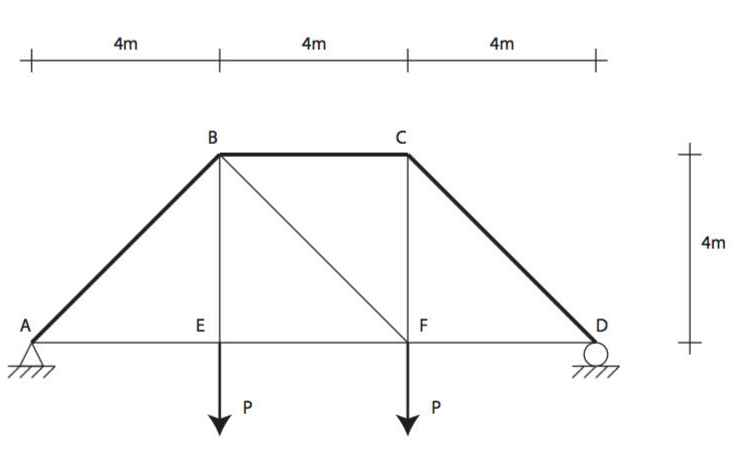
\includegraphics[width=0.8\textwidth]
    {examples/fig_quofem/truss.png} }
  \caption{Two-dimensional truss model used in Verification.}
  \label{fig:truss}
\end{figure}

\begin{table}[hbt!]                       
  \centering
\begin{adjustbox}{max width=\textwidth}            
  \begin{tabular}{lllll}                    
    \toprule          
      Uncertain Parameter & 	Distribution	 &  Mean  &  Standard Deviation \\ \hline
	Elastic Moduli $[kN/mm^2]$	 & Normal & 	205	 & 15 \\ \hline
	Load $[kN]$ & 	Normal	 & 25	 & 2.5 \\ \hline
  Cross section area (upper) $[mm^2]$ & Normal &   500  & 25 \\ \hline
  Cross section area (lower) $[mm^2]$ & Normal &   250  & 10 \\ \hline
  \end{tabular}
\end{adjustbox}
  \caption{Uncertain parameters defined in the portal frame model}             
  \label{tab:uncertainty}                 
\end{table}

We assume that the random variables are independent (i.e., zero covariance), and aim to estimate the mean and standard deviation of the vertical displacement at point F, with $95\%$ confidence intervals for both statistics. In this example, Dakota was used in conjunction with OpenSees. The setup example problem, populated entries, and sample results are show in the following figures.


Figures \Cref{fig:basic}, \Cref{fig:correlation}, \Cref{fig:cdfp}, \Cref{fig:cdfoutput}, and \Cref{fig:psamples} show the results corresponding to the forward problem, including sampling and surrogate-based. 

\begin{figure}[!htbp]
  \centering {
    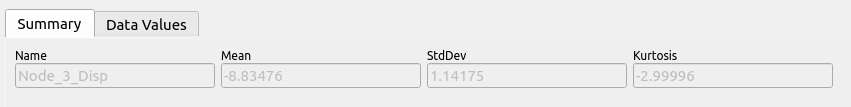
\includegraphics[width=0.8\textwidth]
    {examples/fig_quofem/basic_summary.png} }
  \caption{Basic summary statistics for the specified output. }
  \label{fig:basic}
\end{figure}

\begin{figure}[!htbp]
  \centering {
    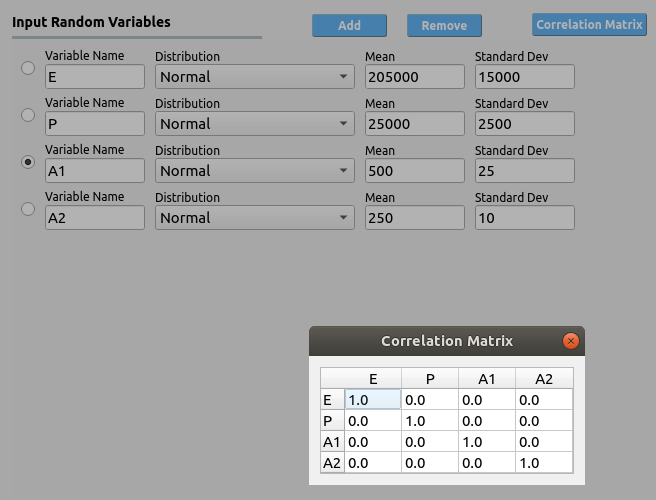
\includegraphics[width=0.8\textwidth]
    {examples/fig_quofem/correlation.png} }
  \caption{Input panel for the correlation matrix for the random variables of the truss problem. }
  \label{fig:correlation}
\end{figure}

\begin{figure}[!htbp]
  \centering {
    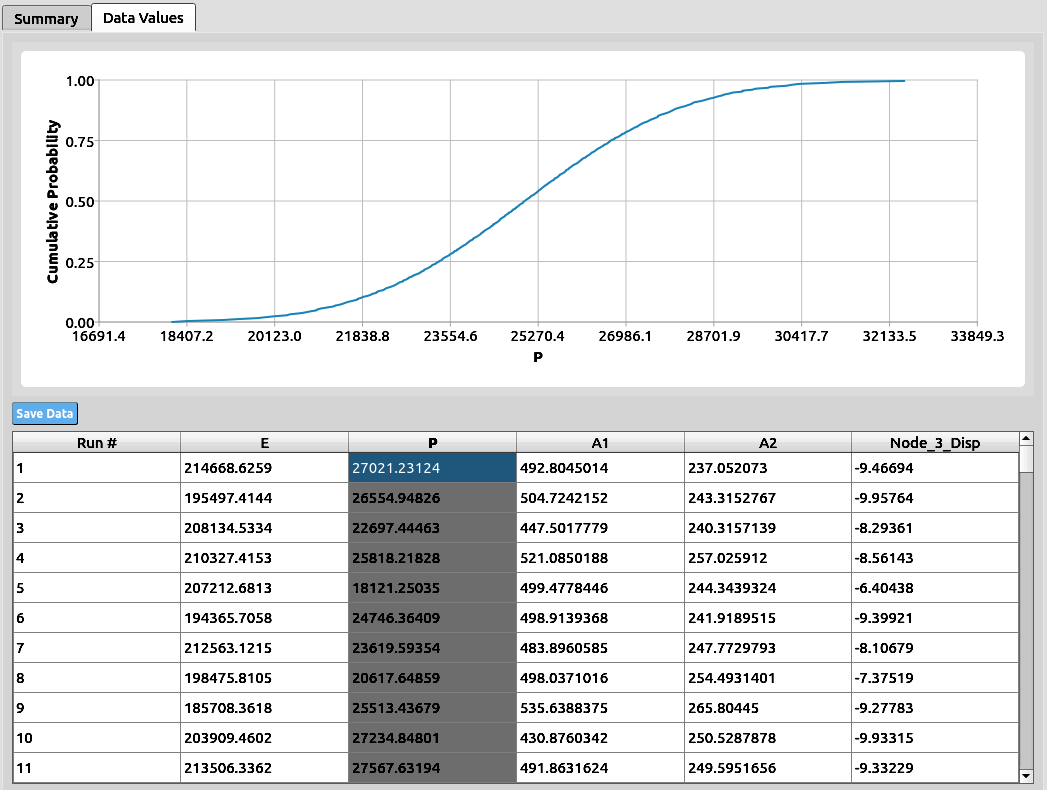
\includegraphics[width=0.8\textwidth]
    {examples/fig_quofem/p_cdf.png} }
  \caption{Samples of the random variables P along with the corresponding Cumulative Distribution Function for the truss problem. }
  \label{fig:cdfp}
\end{figure}

\begin{figure}[!htbp]
  \centering {
    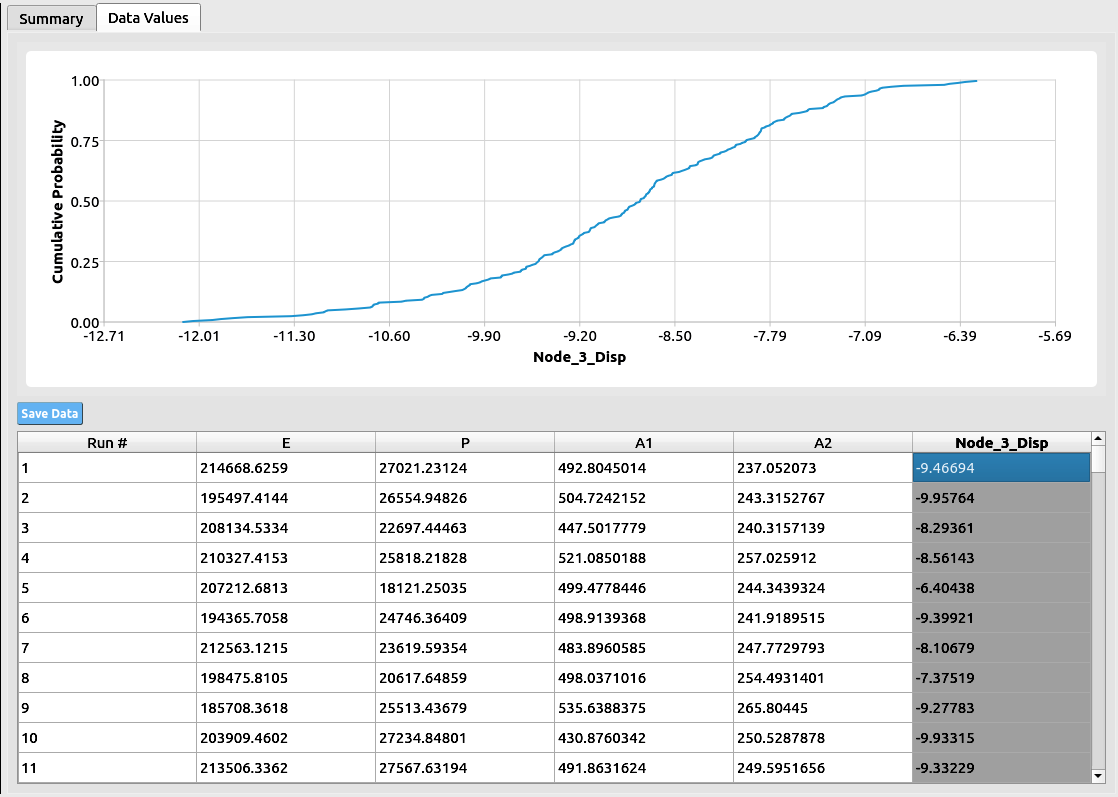
\includegraphics[width=0.8\textwidth]
    {examples/fig_quofem/qoi_cdf.png} }
  \caption{Samples of the output variable along with the corresponding Cumulative Distribution Function for the 2D truss problem. }
  \label{fig:cdfoutput}
\end{figure}

\begin{figure}[!htbp]
  \centering {
    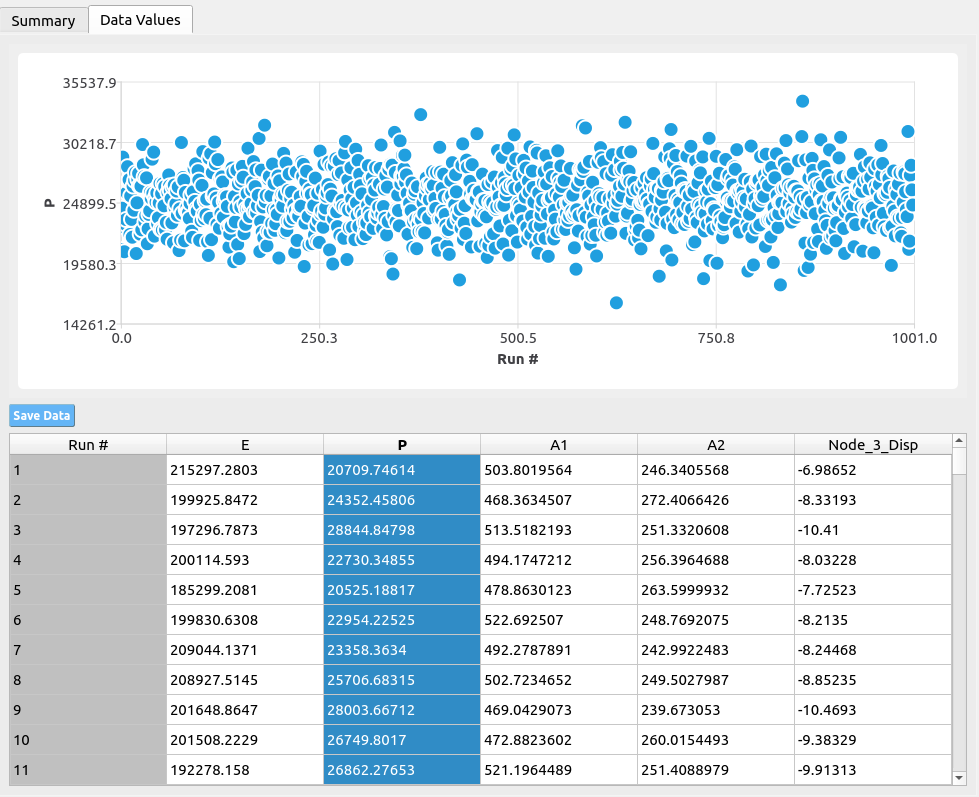
\includegraphics[width=0.8\textwidth]
    {examples/fig_quofem/run_plot.png} }
  \caption{Scatter plot of samples of the random variable P. }
  \label{fig:psamples}
\end{figure}
